\documentclass[10pt,twocolumn,letterpaper]{article}

\usepackage{cvpr}
\usepackage{times}
\usepackage{epsfig}
\usepackage{graphicx}
\usepackage{amsmath}
\usepackage{amssymb}
\usepackage{booktabs}

% Include other packages here, before hyperref.

% If you comment hyperref and then uncomment it, you should delete
% egpaper.aux before re-running latex.  (Or just hit 'q' on the first latex
% run, let it finish, and you should be clear).
\usepackage[breaklinks=true,bookmarks=false]{hyperref}

\cvprfinalcopy % *** Uncomment this line for the final submission

\def\cvprPaperID{****} % *** Enter the CVPR Paper ID here
\def\httilde{\mbox{\tt\raisebox{-.5ex}{\symbol{126}}}}

% Pages are numbered in submission mode, and unnumbered in camera-ready
%\ifcvprfinal\pagestyle{empty}\fi
\setcounter{page}{1}
\begin{document}

%%%%%%%%% TITLE
%\title{CAFA-like Protein Functional Annotation Prediction with Hybrid Convolutional Long Short-Term Memory Recurrent Neural Networks}

\title{CAFA-like Protein Biological Function Prediction by Leveraging ProtT5 PLM Embeddings and Deep Feed-Forward Neural Networks}

\author{
Marco Uderzo\\
{\small Department of Mathematics, University of Padua}\\
{\tt\small marco.uderzo@studenti.unipd.it}\\
{\tt\small ID: 2096998} \\
\and
Tanner Graves\\
{\small Department of Mathematics, University of Padua}\\
{\tt\small tanneraaron.graves@studenti.unipd.it}\\
{\tt\small ID: 2073559} \\
\and
Claudio Palmeri \\
{\small Department of Mathematics, University of Padua}\\
{\tt\small claudio.palmeri@studenti.unipd.it}\\
{\tt\small ID: 2062671} \\
}


\maketitle
%\thispagestyle{empty}


%%%%%%%%% ABSTRACT
\begin{abstract}
    The prediction of the biological function of proteins has been a fundamental topic of bioinformatics. Performing the wet-lab experiments 
    to determine these functions is very expensive and time consuming, so it is crucial to develop computational 
    methods for automated function prediction. Gene Ontology is a standardized system to categorize and describe function 
    in a hierarchical manner.
    This paper concerns the development and evaluation of a Deep Learning model to predict the biological function of proteins, especially by leveraging the per-protein embeddings generated the ProtT5 Protein Language Model.
\end{abstract}

%%%%%%%%% BODY TEXT
\section{Introduction}

\subsection{Protein Biological Function Prediction}
Proteins are responsible for many activities in our tissues, organs, and bodies and they also play a central role in the structure and function of cells.
The accurate assignment of biological function to the protein is key to understanding life at the molecular level. However, assigning function to any 
specific protein can be made difficult due to the multiple functions many proteins have, along with their ability 
to interact with multiple partners. More knowledge of the functions assigned to proteins, potentially aided by Data Science, could 
lead to curing diseases and, overrall, drastically improving human health.\\

Gene Ontology is a standardized system to categorize and describe function in a hierarchical manner.
In order to categorize and classify functions, Gene Ontology has separated the functions into 3 sub-ontologies:
\begin{itemize}
\item {\bf Molecular Function}: functions that the protein performs at the molecular level.
\item {\bf Biological Process}: events or processes that the protein is involved in.
\item {\bf Cellular Component}: locations in the cell that the protein is active. 
\end{itemize}
These sub-ontologies are completely separated from each other, and the terms in them do not have inter-relations between them. \\

Overall, this project concerns the development and evaluation of a Deep Learning model to predict the biological function of proteins.



\subsection{Simplifications from CAFA}
As specified in the project requirements, in order to make the task manageable in terms of computational complexity, some simplifications were made.
\begin{itemize}
\item Only functions that have more than 50, 250, 50 instances respectively in Molecular Function (MF), Biological Process (BP), and Cellular Componet (CC) have been gathered. 
\item Proteins with sequence length of more than 2000 have been removed.
\item Only functional annotations with experimental evidence code, TAS, and IC have been considered.
\end{itemize}


\section{Methods}

\subsection{Training Dataset Description}

The full training dataset for the project contains the following files:

\begin{itemize}
    \item \textit{train\_set.tsv}: The proteins, their Gene Ontology (GO) annotations, and their corresponding aspects are given in a tab-separated file. The GO annotations that are given for each protein are already propagated to the root of the ontology.

    \item \textit{train\_ids.txt}: This file contains the accession IDs of the proteins that are given. It contains about 123,000 proteins.

    \item \textit{train.fasta}: This file contains the sequence of the train proteins in FASTA format.

    \item \textit{train\_embeddings.h5}: This file contains ProtT5 embeddings for each protein in the train set.

    \item \textit{train\_protein2ipr.dat}: This file contains the InterPro domains for proteins of the training set.

    \item \textit{go-basic.obo}: This file contains the whole Ontology terms and the relationships between them. Note that the only relationships that we consider are \texttt{part\_of} and \texttt{is\_a}.
\end{itemize}

In our project we are not using all of these files. For brevity, we now describe more in detail the data we decided to use as our final training set.


\subsubsection{Gene Ontology Annotations and Aspects}

Gene Ontology provides a framework for the representation of gene and gene product attributes across all species. In our file, each protein is annotated with relevant GO terms. These annotations describe the roles of proteins at various levels, such as their biological processes, cellular components, and molecular functions.

By visualizing the distribution of GO\_terms in our train\_set.tsv file, we realize that the data is massively unbalanced (?), with some terms being overrepresented, where as most are underrepresented, creating a long-tail scenario.

\begin{center}
    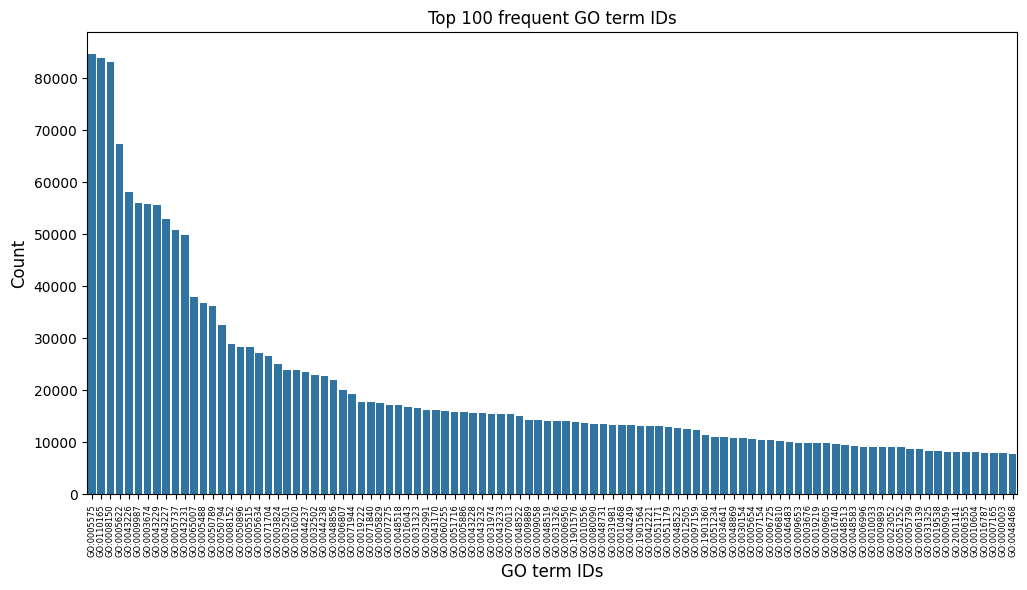
\includegraphics[scale=0.25]{img/go_terms_distribution.png} \\
\end{center}


\subsubsection{ProtT5 PLM Embeddings}

ProtT5 is an advanced language model specifically designed for processing and interpreting protein sequences. Developed as an extension of the T5 (Text-to-Text Transfer Transformer) framework, ProtT5 is able to capture the complex patterns and structures inherent in protein sequences.
ProtT5 embeddings are vector representations of protein sequences generated by the ProtT5 model. These embeddings encapsulate the contextual information of amino acids in a protein sequence, effectively representing the sequence in a high-dimensional space.

\subsection{Dataset Preprocessing}

Protein IDs and their aspect and GO\_term are loaded from the tsv train\_set.tsv file, and for each protein, its embeddings in .h5 format are also parsed. Each embedding consists in 1024 columns.


\subsection{Model Development}

Our training data contains mostly tabular data, except the FASTA protein sequences. Though, we already have embeddings from the ProtT5 Protein Language Model, which is based on the Transformer architecture, known for its efficacy in dealing with long time-space-dependent data. Therefore, using more advanced architecture like RNNs to deal with the raw FASTA sequences would most likely not yield any better result than a Deep Neural Network. RNN-based models could have been leveraged in case we had at our disposal per-residue ProtT5 embeddings, instead of just per-protein embeddings. \\



A summary of the model's architecture is shown below.

\begin{center}
\begin{tabular}{lccc}
    \toprule
    Layer Type & Output Shape & Param \# & Activation\\
    \midrule
    Dense & (None, 128) & 131200 & ReLU\\
    Dropout & (None, 128) & 0 & N/A\\
    Dense &  (None, 256) & 33024 & ReLU \\
    Output\_cc & (None, 625) & 320625 & Sigmoid \\
    \bottomrule
\end{tabular} \\
\end{center}

%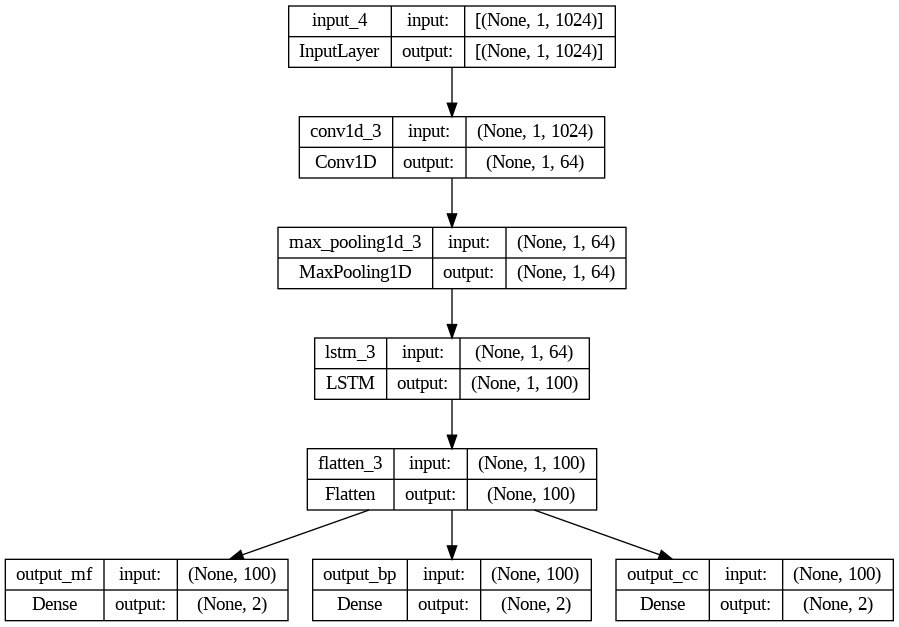
\includegraphics[scale=0.25]{img/model_diagram.png} \\

The hyperparameters of the model are listed in the following table. \\

\begin{center}
\begin{tabular}{lcc}
    \toprule
    Hyperparameter & Value \\
    \midrule
    Learning Rate & 0.001 \\
    Epochs & 50 \\
    Batch Size & 32 \\
    Optimizer & Adam \\
    Loss Function & Binary Cross-Entropy\\
    \bottomrule
\end{tabular} \\
\end{center}


\section{Results}

\subsection{Performance Evaluation}

\section{Discussion}

\section{Usage Overview}

\section{Code Availability}
The datasets used and all the code used for this project is available
at the following \href{https://github.com/marcouderzo/BioData-ProteinFunctionPrediction}{GitHub Repository}.



%-------------------------------------------------------------------------
\section{References}

List and number all bibliographical references in 9-point Times,
single-spaced, at the end of your paper. When referenced in the text,
enclose the citation number in square brackets, for
example.  Where appropriate, include the name(s) of
editors of referenced books.

%{\small
%\bibliographystyle{ieee_fullname}
%\bibliography{egbib}
%}

\end{document}
